\section{Introduction}
\label{sec:intro}

\begin{enumerate}
	\item C-RAN is the future, where functions of BBUs are implemented in a centralized and virtualized way;
	\item \fixit{Two concerns are not checked yet: a) how to assess resource requirement and evaluate tolerance of DT task? b) how to queue and perform selection action? }
	\item In this paper, we propose a novel framework where both BBU tasks and general edge computing tasks are processed simultaneously in a homogeneous edge cloud with general-purposed processors.
	\item By applying resource split between vBBU and vMC, the resource split between DT and CT is implemented. \fixit{So, why not just split computation resource for DT and CT?} 
\end{enumerate}

\begin{figure*}[htb!]
	\centering
	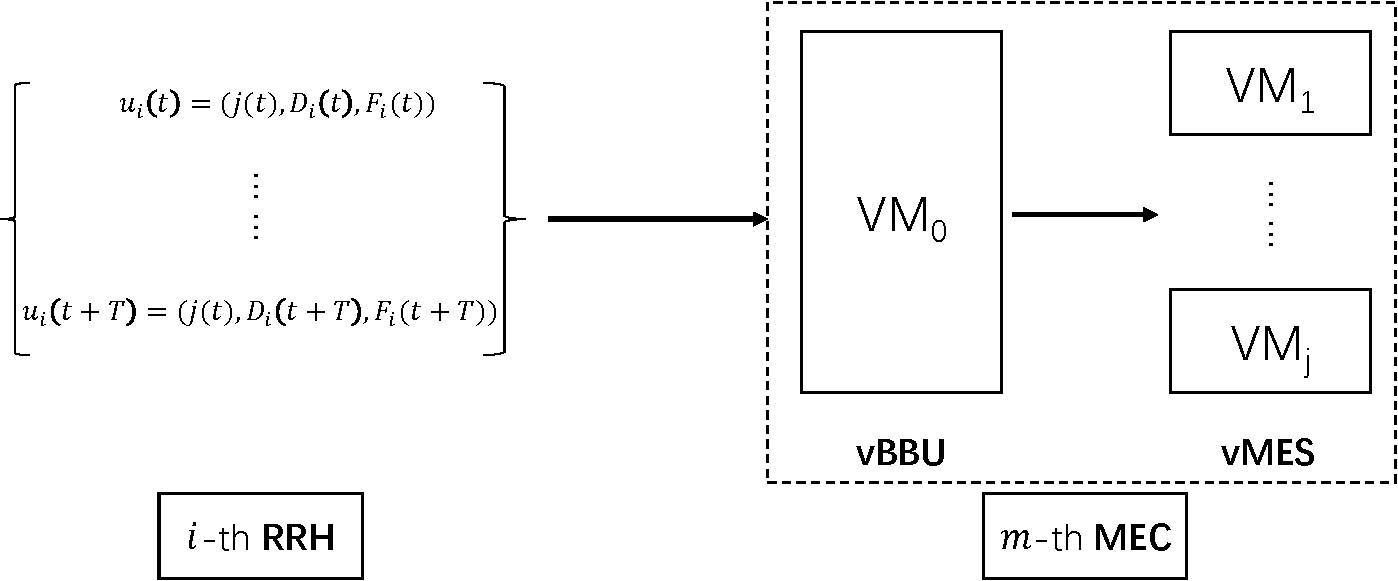
\includegraphics[width=0.9\textwidth]{images/cran-system-model.pdf}
	\caption{The Illustration of System Model.}
	\label{fig:scenario}
\end{figure*}